%\documentclass[11pt,english,ngerman,pointlessnubers, abstraction, headsepline,liststotoc]{scrreprt}
%\documentclass[11pt]{report}
\documentclass[11pt,ngerman,titlepage,oneside, headsepline,listof=totoc]{scrreprt}
\usepackage[a4paper]{geometry}
%\geometry{verbose, tmargin=3cm, bmargin=3cm, lmargin=3.25cm, rmargin=2.5cm, headheight=1cm, headsep=0.666cm, footskip=1cm}
\usepackage[T1]{fontenc}
\usepackage[german]{babel}
\selectlanguage{german}
\usepackage[utf8x]{inputenc}

\usepackage{lmodern}
\renewcommand{\sfdefault}{lmss}
\renewcommand{\ttdefault}{lmtt}
%\usepackage{booktabs}
\usepackage{amsmath}
%\usepackage{syntax}
\usepackage{amsfonts}
\usepackage{amssymb}
\usepackage{amsthm}
\usepackage{graphicx}
\usepackage{empheq}
\usepackage{url}
\usepackage{footmisc}
\usepackage{tabularx}
\usepackage[table]{xcolor}
%\usepackage{relsize}
\usepackage{setspace}
%\setstretch{1.4}
\usepackage{caption}
\usepackage{xcolor}
\usepackage{listings}
\usepackage{nameref}
\usepackage{varwidth}
\usepackage{enumitem}
\usepackage{tikz}
\usetikzlibrary{positioning,automata,shapes}
\usetikzlibrary{positioning}
\usetikzlibrary{decorations.text}
\usetikzlibrary{decorations.pathmorphing,backgrounds,calc}
\usetikzlibrary{decorations.pathreplacing,angles,quotes}
\usetikzlibrary{shapes,arrows,external,shapes.callouts}
	\tikzstyle{element} = [rectangle, font=\fontsize{0.75em},font=\footnotesize, draw, text centered, minimum height=8mm, minimum width=15mm]
	\definecolor{light-gray}{gray}{0.98}
	\definecolor{CPgray}{gray}{0.96}
	\colorlet{macBorder}{black!25}
	\colorlet{dataBorder}{black!50}
	%\definecolor{macBorder}{RGB}{53,125,145}
	%\definecolor{dataBorder}{RGB}{133,137,63}
	\tikzstyle{macElement} = [rectangle, font=\footnotesize, draw, text centered, minimum height=12mm, minimum width=30mm,text=black]
	\tikzstyle{macElementField} =[macElement, color=macBorder,  text centered, text width=27mm, line width=2pt,text=black]
	\tikzstyle{macElementDeteil} =[macElement, color=macBorder, text centered, text width=25mm, minimum height=12mm,  line width=1pt,text=black]
	\tikzstyle{dataElementField} =[macElement, color=dataBorder,  text centered, text width=27mm, line width=2pt,text=black]
	\tikzstyle{dataElementDeteil} =[macElement, color=dataBorder, text centered, text width=25mm, minimum height=12mm, line width=1pt,text=black]
	
	
\usepackage{caption}
\usepackage{subcaption}
\usepackage{float}
\usepackage{wrapfig}
\usepackage{multirow}
\usepackage{ragged2e}
\usepackage{array}
\usepackage{longtable}
\usepackage[export]{adjustbox} %used for image alignment on title page
%\floatstyle{boxed}
%\restylefloat{figure}

\lstdefinestyle{BashInputStyle}{
	language=sh,
	basicstyle=\small\sffamily,
	numbers=left,
	numberstyle=\tiny,
	breaklines=true,
	numbersep=3pt,
	frame=tb,
	columns=fullflexible,
	backgroundcolor=\color{yellow!20},
	linewidth=0.9\linewidth,
	xleftmargin=0.1\linewidth
}
\colorlet{punct}{red!60!black}
\definecolor{background}{HTML}{EEEEEE}
\definecolor{delim}{RGB}{20,105,176}
\colorlet{numb}{magenta!60!black}

\lstdefinelanguage{json}{
    basicstyle=\normalfont\ttfamily,
    numbers=left,
    numberstyle=\scriptsize,
    stepnumber=1,
    numbersep=8pt,
    showstringspaces=false,
    breaklines=true,
    frame=lines,
    backgroundcolor=\color{background},
    literate=
     *{0}{{{\color{numb}0}}}{1}
      {1}{{{\color{numb}1}}}{1}
      {2}{{{\color{numb}2}}}{1}
      {3}{{{\color{numb}3}}}{1}
      {4}{{{\color{numb}4}}}{1}
      {5}{{{\color{numb}5}}}{1}
      {6}{{{\color{numb}6}}}{1}
      {7}{{{\color{numb}7}}}{1}
      {8}{{{\color{numb}8}}}{1}
      {9}{{{\color{numb}9}}}{1}
      {:}{{{\color{punct}{:}}}}{1}
      {,}{{{\color{punct}{,}}}}{1}
      {\{}{{{\color{delim}{\{}}}}{1}
      {\}}{{{\color{delim}{\}}}}}{1}
      {[}{{{\color{delim}{[}}}}{1}
      {]}{{{\color{delim}{]}}}}{1},
}

 \usepackage[nounderscore]{syntax}
 \newenvironment{BNF}{\captionsetup{type=lstlisting}}{}
 
\usepackage{acronym}
\setcounter{secnumdepth}{3}
\setcounter{tocdepth}{3}
%\setcounter{tocdepth}{5}
%\setcounter{secnumdepth}{4}

%\usepackage{titlesec}

\usepackage[Algorithmus]{algorithm}
\usepackage[noend]{algpseudocode}
\usepackage[titletoc,title]{appendix}
\usepackage[nottoc]{tocbibind}

\newcommand{\reftablle}[1]{\textit{Tabelle \ref{#1}, \nameref{#1}, }}
\newcommand{\reftablleb}[1]{\textit{Tabelle \ref{#1}, \nameref{#1}}}
\newcommand{\reftabllec}[1]{\textit{Tabelle \ref{#1}}}
\newcommand{\refabb}[1]{\textit{Abbildung \ref{#1}}}
\newcommand{\refabschnitt}[1]{\textit{Abschnitt \ref{#1}: \nameref{#1}}}
\newcommand{\refabschnittb}[1]{\textit{Abschnitt \ref{#1}}}
\newcommand{\refunterabschnitt}[1]{\textit{Unterabschnitt \ref{#1}}}
\newcommand{\refuntuntererabschnitt}[1]{\textit{Unterunterabschnitt \ref{#1}}}
\newcommand{\reflisting}[1]{\textit{Listing \ref{#1}}}
\newcommand{\refalgo}[1]{\textit{Algorithmus \ref{#1}}}
\newcommand{\refanhang}[1]{\textit{Anhang \ref{#1}}}
\renewcommand{\listalgorithmname}{Algorithmenverzeichnis}


\begin{document}
% Hintergründe, Grundlagen, Unterteilung des Dokuments in Abschnitte (Client/Server, UART, Funk, LC)
% Client/Server Struktur
% Python-Skript und UART Kommunikation
% Funkkommunikation und LCs
\begingroup
  %\renewcommand*{\chapterpagestyle}{empty}
  \pagestyle{plain}
	\setcounter{page}{1}
	\pagenumbering{roman}
  \tableofcontents
  \clearpage
\endgroup
\pagenumbering{arabic}
\pagestyle{plain}
\setcounter{page}{1}
\section{Datenmodel Beispiele}
\subsection{Benutzer(Datenmodelle)}
\begin{lstlisting}[caption={Beispiel 1 Schüler},frame=tlrb]
{
 id: "USER-01",
 name: "Leming",
 surename: "Zobel",
 birtdate: "03-01-2003",
 sex: "mail",
 rols: [
 {
  school_id: "SCHULE-01",
	role: "students",
	start: "01-09-2009",
	end: "31-08-2016",
	school-years: ["SJ-09/10","SJ-10/11","SJ-11/12","SJ-13/14","SJ-14/15","SJ-15/16"]
 }, {
  school_id: "SCHULE-04",
	role: "students",
	start: "01-09-2016",
	school-years: ["SJ-16/17","SJ-17/18","SJ-18/19","SJ-19/20","SJ-20/21"]
 },{
  school_id: "SCHULE-02",
	role: "external-students",
	start: "01-09-2019",
	end: "31-08-2020",
	school-years: ["SJ-19/20"]
 },
 ],
 guardians [
 {
	user_id: "USER-02",
	start: "01-09-2009",
	end: "03-01-2020",
 },  {
	user_id: "USER-04",
	start: "01-09-2009",
	end: "03-01-2020",
 }
 ],
}
\end{lstlisting}
\lstset{
  language=json,
  tabsize=2,
  captionpos=b,
  numbers=left,
  commentstyle=\color{green},
  backgroundcolor=\color{white},
  numberstyle=\color{gray},
  keywordstyle=\color{blue} \textbf,%otherkeywords={xdata},
  keywordstyle=[2]\color{red}\textbf,
  identifierstyle=\color{black},
  stringstyle=\color{red}\ttfamily,
  basicstyle = \ttfamily \color{black} \footnotesize,
  showstringspaces=false,
	breakatwhitespace=false,         % sets if automatic breaks should only happen at whitespace
  breaklines=true, 
}
\begin{lstlisting}[caption={Beispiel für Benutzer mit Rollen \"teachers\" und \"guardians\"},frame=tlrb]
{
 id: "USER-02",
 name: "Altes Leming 1",
 surename: "Zobel",
 birtdate: "03-01-2003",
 sex: "female",
 assignments: [
 {
  school_id: "SCHULE-01",
	role: "guardians",
	start: "01-09-2009",
	end: "31-08-2016",
	school-years: ["SJ-09/10","SJ-10/11","SJ-11/12","SJ-13/14","SJ-14/15","SJ-15/16"]
 }, {
  school_id: "SCHULE-04",
	role: "guardians",
	start: "01-09-2016",
	school-years: ["SJ-16/17","SJ-17/18","SJ-18/19","SJ-19/20","SJ-20/21"]
 }, {
  school_id: "SCHULE-02",
	role: "guardians",
	start: "01-09-2019",
	end: "31-08-2020",
	school-years: ["SJ-19/20"]
 }, {
  school_id: "SCHULE-02",
	role: "teacher",
	start: "01-09-2019"
 }
 ],
 childs: [
 {
	user_id: "USER-01",
	start: "01-09-2009",
	end: "03-01-2020",
 },  {
	user_id: "USER-03",
	start: "01-09-2009",
	end: "03-01-2020",
 }
 ],
 classes: [
  {
	 class_id: "KLASSE-0031",
   school_id: "SCHULE-02",
	 school-year: "SJ-09/10",
	 start: "01-09-2009",
	 end: "31-08-2010",
	}, {
	 class_id: "KLASSE-0032",
   school_id: "SCHULE-02",
	 school-year: "SJ-20/21",
	 start: "01-09-2020",
	 end: "31-08-2021",
	}, {
	 class_id: "KLASSE-0033",
   school_id: "SCHULE-02",
	 school-year: "SJ-20/21",
	 start: "01-09-2020",
	 end: "31-08-2021",
	}, 
 ]
}
\end{lstlisting}
\input{datamodel/user_03}
\input{datamodel/user_04}
\input{datamodel/user_05}
\lstset{
  language=json,
  tabsize=2,
  captionpos=b,
  numbers=left,
  commentstyle=\color{green},
  backgroundcolor=\color{white},
  numberstyle=\color{gray},
  keywordstyle=\color{blue} \textbf,%otherkeywords={xdata},
  keywordstyle=[2]\color{red}\textbf,
  identifierstyle=\color{black},
  stringstyle=\color{red}\ttfamily,
  basicstyle = \ttfamily \color{black} \footnotesize,
  showstringspaces=false,
	breakatwhitespace=false,         % sets if automatic breaks should only happen at whitespace
  breaklines=true, 
}
\begin{lstlisting}[caption={Beispiel 1 Schüler},frame=tlrb]
{
 subject_id: "SUBJECT-0001",
 name: "Deutsch 1-A"
 subject_ref_id: "DE",
 school_id: "SCHULE-01",
 school-year: "SJ-09/10",
 start: "01-09-2009",
 end: "28-02-2010",
 classes: [ "KLASSE-01","KLASSE-03","KLASSE-05" ],
 grade: [ "1" ],
 students: [
  { 
   user_id: "USER-01",
	 start: "01-09-2009",
	 end: "28-02-2010",
	}, { 
	 user_id: "USER-06",
	 start: "01-09-2009",
	 end: "28-02-2010",
	}, { 
	 user_id: "USER-07",
	 start: "01-09-2009",
	 end: "31-12-2009",
	},
 ]
 time_tabel [
  {
	 day: "1",
	 start: "08:00:00",
	 end: "08:45:00",
	 repeate: "weackly"
  }, {
	 day: "2",
	 start: "08:00:00",
	 end: "08:45:00",
	 repeate: "weackly"
	}, {
	 day: "3",
	 start: "08:50:00",
	 end: "09:35:00",
	 repeate: "beweackly",
	 start: "weack-1"
	}, {
	 day: "4",
	 start: "08:50:00",
	 end: "09:35:00",
	 repeate: "beweackly",
	 start: "weack-2"
	}, {
	 day: "3",
	 start: "08:50:00",
	 end: "09:35:00",
	 repeate: "ontime",
	 date: "30-10-2009"
	}	 
 ]
}
\end{lstlisting}

\chapter{Einleitung und Vorüberlegungen}
Ziel dieses Dokument ist es, eine technische Definition einer REST-API zu schaffen, wie aus einem verbundenen Bildungssystem relevante Daten aus einem IDM-System bezogen werden können.\\
\\
Der IDM-Provider ist verpflichtet, mindestens die geforderten Schnittstellen und Protokolle mit der angegebenen Verfügbarkeitsanforderung bereitzustellen. 
Im Gegenzug erhält der IDM-Provider über viele Objekte die Hoheit der zentralen ID-Vergabe. 
Eine zentralisierte ID-Vergabe ist notwendig, damit verschiedene nachgelagerte Bildungssysteme (z.B. Schulverwaltungssoftwares, Lernplattformen) interoperabel sind.\\
\\
Es werden die notwendigen Endpunkte definiert und jeweils die zugelassenen Operationen nebst verwendeter HTTP-Methode festgelegt.

\section{Benutzerrollen}
\label{Benutzerrollen}
An dieser Stelle listen wir eine Reihe von im Kontext "'Schule"' bekannten Rollen auf, die auf IDM-Provider-Seite definiert und im Client für die Berechtigungssteuerung genutzt werden können.
\\


\begin{table}[htb]
	\begin{tabularx}{\textwidth}{|c|X|}
		\hline
\textbf{Rollenname} & \textbf{Beschreibung der Rolle} \\ \hline
guest & Gäste und nicht authentifizierte Benutzer \\ \hline
user & authentifizierte Benutzer \\ \hline
student & Schüler \\ \hline
external-student & Schüler von anderen Schulen, die nur einzelne Fächer oder Kurse besuchen \\ \hline
guardian & Eltern, Erziehungsberechtigte, Vormünder von Schülern \\ \hline
teacher & Lehrkräfte \\ \hline
external-expert & Externe Experten zur Unterstützung des Unterrichts (auch Schulassistenten und pädagische Mitarbeiter) \\ \hline
principal & Schulleitung \\ \hline
school-admin & Schul-Administrator \\ \hline
school-board & Schulträger \\ \hline
fed-school-board & Mitarbeiter/-in des Schulministeriums \\ \hline
sync-system & Systeme, welchen ein Sync mit allen Daten erlaubt ist \\ \hline

	\end{tabularx}

		\caption{Mögliche Benutzerrollen im Kontext "Schule"}
		\label{tab:intro:roles}
\end{table}

Bei Bedarf können IDM-Provider und Client weitere Rollen festlegen, die additiv zu vergeben und nicht Teil dieser Konzeption sind.

\chapter{Authentifizierung und Autorisierung}
Um den Zugriff auf Client und REST-API gleichermaßen zu steuern und dabei im Client keine Anmeldeinformationen vorhalten zu müssen, wird eine Authentifizierung und Autorisierung per \textit{OAuth2-Protokoll} und \textit{OpenID Connect} vorgeschrieben.

\subsection{OAuth2}
\label{auth:oauth2}

OAuth2 ist eine Spezifikation, wie \textit{Access Tokens} ausgegeben werden (RFC 6749, s. https://tools.ietf.org/html/rfc6749). 

Der Autorisierungsserver des IDM-Providers muss gemäß RFC 6749 folgende Endpunkte bereitstellen:

\begin{table}[htb]
    \begin{tabularx}{\textwidth}{|c|X|}
        \hline
\textbf{Endpunkt} & \textbf{Funktion des Endpunkts} \\ \hline
Authorization & Initiierung der Autorisierung und Benutzerzustimmung durch parametrisierten Aufruf \\ \hline
Token & Liefert gegen Authorization Code Access Token zurück \\ \hline
    \end{tabularx}

        \caption{Endpunkte, die durch den IDM-Provider für die Anmeldung per OAuth2 zur Verfügung gestellt werden müssen}
        \label{tab:auth:endpoints}
\end{table}

OAuth2 definiert sogenannte \textit{Grant Types}, die vom \textit{Client} über das Setzen eines oder mehrerer \textit{respond_type} beim Aufruf des \textit{Authorization Endpoint} gewählt werden können. 
Diese \textit{Grant Types} beschreiben Möglichkeiten, wie ein Client einen \textit{Access Token} erlangt, über den im Namen des Benutzers anschließend eine API aufgerufen werden kann. 
Während \textit{respond_type=code} den \textit{Authorization Code Grant} initiiert, liefert \textit{respond_type=token} den Access Token direkt nach Autorisierung zurück. 
Zudem lassen sich über \textit{Access Token Scopes} vom Client Anwendungsbereiche des vom Autorisierungsserver gelieferten Access Tokens anfordern (s. https://datatracker.ietf.org/doc/html/rfc6749#section-3.3).

Die \textit{Internet Engineering Task Force (IETF)} empfiehlt als Best-Practice-Ansatz die Verwendung des \textit{Authorization Code Grant} (s. https://datatracker.ietf.org/doc/html/draft-ietf-oauth-security-topics#section-2.1.1). 
Je nachdem, ob es sich um einen \textit{Confidential} oder \textit{Public Client} handelt, d.h., ob ein \textit{Client Secret} verwendet werden kann, wird ein \textit{Proof Key for Code Exchange (PKCE)} empfohlen bzw. vorgeschrieben. 
Der PKCE ist eine Erweiterung des \textit{Authorization Code Grant}, um Cross-Site-Request-Forgery (CSRF) oder Authentication-Code-Injection-Angriffe zu verhindern (s. https://datatracker.ietf.org/doc/html/rfc7636).

Der Ablauf der Autorisierung per OAuth2-Protokoll im \textit{Authorization Code Grant} ist in Abbildung \refabb{fig:auth-code-grant} dargestellt. 

\begin{figure}[htbp]
\centering
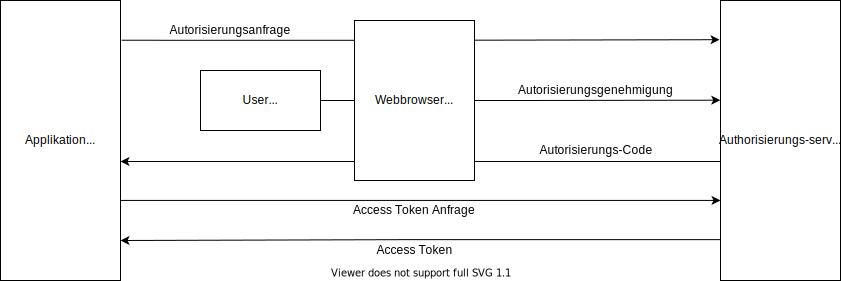
\includegraphics[width=\textwidth]{Authentication_Code_Grant.png}
\caption{Ablauf des Authentication Code Grant}
\label{fig:auth-code-grant}
\end{figure}

Der Ablauf wird durch den \textit{Client} gestartet, gefolgt von der Authentifizierung des \textit{Resource Owners} beim Autorisierungserver. 
Der Autorisierungserver sendet einen \textit{Authorization Code} an den \textit{Client}, der diesen wiederum direkt beim Autorisierungsserver gegen den \textit{Access Token} tauscht.

Über den Access Token erhält der Benutzer schließlich Zugriff auf die REST-API.

\subsection{OpenID Connect}
\label{auth:openid}

OpenID Connect ist eine Spezifikation, wie \textit{ID Tokens} mit personenbezogenen Daten ausgegeben werden (s. https://openid.net/specs/openid-connect-core-1_0.html). 
Dabei setzt OpenID Connect auf das OAuth2-Protokoll auf. 
OpenID Connect definiert ein weiteren \textit{response_type=id_token}. 
Dieser ermöglicht es, neben dem Access Token einen \textit{ID Token} vom Autorisierungsserver anzufordern. 
Um OpenID Connect nutzen zu können, muss im in \refabschnitt{auth:oauth2} beschriebenen Autorisierungsprozess der Parameter \textit{Scopes} um \textit{openid} erweitert werden.

Über den ID Token erlangt der Client Zugriff auf personenbezogene Daten des Benutzers. 
\textit{OpenID Connect} definiert eine Reihe von Standard-\textit{claims} (s. https://openid.net/specs/openid-connect-core-1_0.html#StandardClaims), die im \textit{Scope}-Parameter beim Aufruf der Autorisierungs-URL aufgelistet werden und die spezifische Benutzerdaten im ID Token angefordern.

\subsection{Einschränkung der Daten}
\label{auth:limit_data}

Die Spezifikation der REST-API sieht vor, dass die Sichtbarkeit der Daten an den definierten Endpunkte bereits im JSON-Objekt gemäß der Berechtigung des anfragenden Benutzers berücksichtigt ist. 
Die ID des Benutzers im Access Token allein reicht nicht aus, um die Sichtbarkeit der Daten korrekt zu beschränken, da einem Benutzer im IDM mehrere Schule-Rolle-Kombinationen zugewiesen sein können (z.B. an verschiedenen Schulen als Lehrkraft tätig oder an derselben Schule sowohl Lehrkraft als auch Elternteil eines Schülers). 
Daher muss die Information, mit welcher Kombination von Schule und Rolle innerhalb dieser Schule der Aufruf eines REST-API-Endpunkts durchgeführt wird, an den IDM-Provider übermittelt werden. 
Dies geschieht durch die Erweiterung der \textit{Scopes}-Liste um den Scope für die Schule und die Rolle als Parameterübergabe beim Autorisierungsvorgang. 
\reflisting{listing:authorization_request} zeigt einen exemplarischen Aufruf des \textit{Authorization Endpoints} mit Übergabe der \textit{Scopes}.
Die zusätzlichen \textit{Scopes}. für Schule und Rolle sind somit im Access Token hinterlegt und können bei der Generierung des zurückzuliefernden JSON-Objekts verwendet werden.

\begin{lstlisting}[caption={Beispielhafter Aufruf des Authorization Endpoints},label={listing:authorization_request},frame=tlrb]
https://<URl zu Autorisierungsendpunkt>?response_type=code
&client_id=<Identifier von Client-App>
&redirect_uri=<Redirect-URL>
&scope=openid teachers id_schule
&state=<Undurchschaubarer Wert fuer Sicherheitszwecke>
\end{lstlisting}

Ein Sonderfall stellen dabei Benutzerkonten mit der Rolle ''sync-system'' dar. 
Diese haben bei Aufruf eines REST-API-Endpunkts grundsätzlich keine Beschränkung auf eine einzelne Schule. 
Daher muss beim Autosierungsvorgang auch kein \textit{Scope} für die Schule an den Autorisierungsserver übergeben werden.

Sofern für ein Benutzerkonto im IDM mehrere Schule-Rolle-Kombinationen hinterlegt sein können, müssen Schule und Rolle bei Start des Authentifizierungsprozesses gegebenenfalls durch den Benutzer wählbar sein. 
Für einen Schule-Rolle-Wechsel ist eine Neuanmeldung bzw. Aktualisierung des Access Tokens bezüglich der \textit{Scopes} für Schule und Rolle notwendig.
\chapter{REST-API-Definition}
\label{sec:RESTAPIDefinition}

\section{Schnitstellen f�r Schulf�cher}
\label{sec:SchnitstellenFuerSchulfaecher}

\subsection{Endpunkt in der REST-API: /api/school-subjects}
\label{sec:end:rest:api:school-subjects}
Die \reftabllec{tab:end:rest:api:school-subjects:meth} listet die zugelassenen Operationen. 
In der Tabelle <REF> ist eine Liste der vollständigen Fächer enthalten.


\begin{table}[!htbp]
	\begin{tabular}{|c|c|c|}
		\hline
			\textbf{Operation} & \textbf{Zugelassen} & \textbf{HTTP-Methode} \\ \hline
			CREATE & Nicht zugelassen & \\ \hline 
			READ & Zugelassen & GET \\ \hline
			UPDATE & Nicht zugelassen & \\ \hline 
			DELETE & Nicht zugelassen & \\ \hline
	\end{tabular}

		\caption{Zugelassene Operationen auf /api/school-subjects}
		\label{tab:end:rest:api:school-subjects:meth}
\end{table}
\input{rest/school-subjects/get}
\input{rest/school-subjects/create}
\input{rest/school-subjects/update}
\input{rest/school-subjects/delete}


\section{Schnittstellen für Schuljahre}

\subsection{Endpunkt in der REST-API: /api/school-years}
\label{sec:end:rest:api:school-years}
Die \reftabllec{tab:end:rest:api:school_years:meth} listet auf, welche Operationen zugelassen sind und welche HTTP-Methoden dabei verwendet werden. 


\begin{table}[!htbp]
	\begin{tabular}{|c|c|c|}
		\hline
			\textbf{Operation} & \textbf{Zugelassen?} & \textbf{HTTP-Methode} \\ \hline
			CREATE & Nein & \\ \hline 
			READ & Ja & GET \\ \hline
			UPDATE & Nein & \\ \hline 
			DELETE & Nein & \\ \hline
	\end{tabular}

		\caption{Zugelassene Operationen auf /api/school-years}
		\label{tab:end:rest:api:school_years:meth}
\end{table}
\section{Schnittstellen für Schulen}


\subsection{Endpunkt in der REST-API: /api/schools}
\label{sec:end:rest:api:schools}
An diesem Endpunkt werden Informationen zu Schulen verarbeitet. Eine Schule beschreibt eine Institution, an der Personen in von Gruppen mit verschiedenen Rollen (s. \refabschnitt{sec:end:rest:api:classes}) an der Unterrichtsdurchführung (s. \refabschnitt{sec:end:rest:api:subjects}) beteiligt sind.

Die \reftabllec{tab:end:rest:api:schools:meth} listet auf, welche Operationen zugelassen sind und welche HTTP-Methoden dabei verwendet werden. 


\begin{table}[!htbp]
	\begin{tabular}{|c|c|c|}
		\hline
			\textbf{Operation} & \textbf{Zugelassen?} & \textbf{HTTP-Methode} \\ \hline
			CREATE & Nein & \\ \hline 
			READ & Ja & GET \\ \hline
			UPDATE & Nein & \\ \hline 
			DELETE & Nein & \\ \hline
	\end{tabular}

		\caption{Zugelassene Operationen auf /api/schools}
		\label{tab:end:rest:api:schools:meth}
\end{table}
\subsection{Endpunkt in der REST-API: /api/schools/\$id}
Die \reftabllec{tab:end:rest:api:schools:id:meth} listet auf, welche Operationen zugelassen sind und welche HTTP-Methoden dabei verwendet werden. 

\begin{table}[!htbp]
	\begin{tabular}{|c|c|c|}
		\hline
			\textbf{Operation} & \textbf{Zugelassen?} & \textbf{HTTP-Methode} \\ \hline
			CREATE & Nein & \\ \hline 
			READ & Ja & GET \\ \hline
			UPDATE & Nein & \\ \hline 
			DELETE & Nein & \\ \hline
	\end{tabular}

		\caption{Zugelassene Operationen auf /api/schools/\$id}
		\label{tab:end:rest:api:schools:id:meth}
\end{table}
\subsection{Endpunkt in der REST-API: /api/schools/\$id/users}
Die \reftabllec{tab:rest:api:schools:id:users:meth} listet auf, welche Operationen zugelassen sind und welche HTTP-Methoden dabei verwendet werden. 
\$id ist die ID der Schule im IDM, auf welche die nachfolgenden Operationen ausgeführt werden.

\begin{table}[!htbp]
	\begin{tabular}{|c|c|c|}
		\hline
			\textbf{Operation} & \textbf{Zugelassen?} & \textbf{HTTP-Methode} \\ \hline
			CREATE & Ja & POST \\ \hline 
			READ & Ja &  \\ \hline
			UPDATE & Ja & POST \\ \hline 
			DELETE & Ja & POST \\ \hline
	\end{tabular}

		\caption{Zugelassene Operationen auf /api/schools/\$id/users}
		\label{tab:rest:api:schools:id:users:meth}
\end{table}

\input{rest/schools/id/users/read}
\input{rest/schools/id/users/create}
\input{rest/schools/id/users/update}
\input{rest/schools/id/users/delete}

\subsection{Endpunkt in der REST-API: /api/schools/\$id/classes}
Die \reftabllec{tab:end:rest:api:schools:id:classes:meth} listet auf, welche Operationen zugelassen sind und welche HTTP-Methoden dabei verwendet werden. 

\begin{table}[!htbp]
	\begin{tabular}{|c|c|c|}
		\hline
			\textbf{Operation} & \textbf{Zugelassen?} & \textbf{HTTP-Methode} \\ \hline
			CREATE & Ja & POST \\ \hline 
			READ & Ja &  \\ \hline
			UPDATE & Ja & POST \\ \hline 
			DELETE & Ja & POST \\ \hline
	\end{tabular}

		\caption{Zugelassene Operationen auf /api/schools/\$id/classes}
		\label{tab:end:rest:api:schools:id:classes:meth}
\end{table}
\subsection{Endpunkt in der REST-API: /api/schools/\$id/subjects}
Die \reftabllec{tab:rest:api:schools:id:subjects:meth} listet auf, welche Operationen zugelassen sind und welche HTTP-Methoden dabei verwendet werden. 

\begin{table}[!htbp]
	\begin{tabular}{|c|c|c|}
		\hline
			\textbf{Operation} & \textbf{Zugelassen?} & \textbf{HTTP-Methode} \\ \hline
			CREATE & Nein & \\ \hline 
			READ & Ja & GET \\ \hline
			UPDATE & Nein & \\ \hline 
			DELETE & Nein & \\ \hline
	\end{tabular}

		\caption{Zugelassene Operationen auf /api/schools/\$id/subjects}
		\label{tab:rest:api:schools:id:subjects:meth}
\end{table}


\section{Schnitstellen für Benutzer}
\label{sec:SchnitstellenFuerBenutzer}

\subsection{Endpunkt in der REST-API: /api/school-years}
\label{sec:end:rest:api:school-years}
Die \reftabllec{tab:end:rest:api:school_years:meth} listet auf, welche Operationen zugelassen sind und welche HTTP-Methoden dabei verwendet werden. 


\begin{table}[!htbp]
	\begin{tabular}{|c|c|c|}
		\hline
			\textbf{Operation} & \textbf{Zugelassen?} & \textbf{HTTP-Methode} \\ \hline
			CREATE & Nein & \\ \hline 
			READ & Ja & GET \\ \hline
			UPDATE & Nein & \\ \hline 
			DELETE & Nein & \\ \hline
	\end{tabular}

		\caption{Zugelassene Operationen auf /api/school-years}
		\label{tab:end:rest:api:school_years:meth}
\end{table}
\subsection{Endpunkt in der REST-API: /api/user/\$id}
Die \reftabllec{tab:end:rest:api:user:id:meth} listet die zugelassenen Methoden. 

\begin{table}[!htbp]
	\begin{tabular}{|c|c|c|}
		\hline
			\textbf{Methode} & \textbf{Zugelassen} & \textbf{HTTP Methode} \\ \hline
			GET & Zugelassen & GET \\ \hline
			UPDATE & Zugelassen & POST \\ \hline 
			CREATE & nicht Zugelassen & \\ \hline  
			DELETE & Nicht Zugelassen & \\ \hline
	\end{tabular}

		\caption{Zugelassen Methoden auf /api/user/\$id}
		\label{tab:end:rest:api:user:id:meth}
\end{table}
\subsection{Endpunkt in der REST-API: /api/user/roles}
Die \reftabllec{tab:end:rest:api:user:roles:meth} listet die zugelassenen Methoden. 

\begin{table}[!htbp]
	\begin{tabular}{|c|c|c|}
		\hline
			\textbf{Methode} & \textbf{Zugelassen} & \textbf{HTTP Methode} \\ \hline
			GET & Zugelassen & GET \\ \hline
			UPDATE & Nicht Zugelassen & \\ \hline 
			CREATE & Nicht Zugelassen & \\ \hline 
			DELETE & Nicht Zugelassen & \\ \hline
	\end{tabular}

		\caption{Zugelassen Methoden auf /api/user/roles}
		\label{tab:end:rest:api:user:roles:meth}
\end{table}
\subsection{Endpunkt in der REST-API: /api/user/roles/\$id}
Die \reftabllec{tab:end:rest:api:user:roles:id:meth} listet auf, welche Operationen zugelassen sind und welche HTTP-Methoden dabei verwendet werden. 

\begin{table}[!htbp]
	\begin{tabular}{|c|c|c|}
		\hline
			\textbf{Operation} & \textbf{Zugelassen?} & \textbf{HTTP-Methode} \\ \hline
			CREATE & Ja & POST \\ \hline 
			READ & Ja & GET \\ \hline
			UPDATE & Ja & POST \\ \hline 
			DELETE & Ja & POST \\ \hline
	\end{tabular}

		\caption{Zugelassene Operationen auf /api/user/roles/\$id}
		\label{tab:end:rest:api:user:roles:id:meth}
\end{table}
\subsection{Endpunkt in der REST-API: /api/user/schools}
Die \reftabllec{tab:end:rest:api:user:schools:meth} listet die zugelassenen Methoden. 

\begin{table}[!htbp]
	\begin{tabular}{|c|c|c|}
		\hline
			\textbf{Methode} & \textbf{Zugelassen} & \textbf{HTTP-Methode} \\ \hline
			GET & Zugelassen & GET \\ \hline
			UPDATE & Zugelassen & POST \\ \hline 
			CREATE & Zugelassen & POST \\ \hline 
			DELETE & Zugelassen & POST \\ \hline
	\end{tabular}

		\caption{Zugelassene Methoden auf /api/user/schools}
		\label{tab:end:rest:api:user:schools:meth}
\end{table}
\subsection{Endpunkt in der REST-API: /api/user/schools/\$id}
Die \reftabllec{tab:end:rest:api:user:schools:id:meth} listet die zugelassenen Methoden. 

\begin{table}[!htbp]
	\begin{tabular}{|c|c|c|}
		\hline
			\textbf{Methode} & \textbf{Zugelassen} & \textbf{HTTP Methode} \\ \hline
			GET & Zugelassen & GET \\ \hline
			UPDATE & Nicht Zugelassen & \\ \hline 
			CREATE & Nicht Zugelassen & \\ \hline 
			DELETE & Zugelassen & POST \\ \hline
	\end{tabular}

		\caption{Zugelassen Methoden auf /api/user/schools/\$id}
		\label{tab:end:rest:api:user:schools:id:meth}
\end{table}
\subsection{Endpunkt in der REST-API: /api/user/classes}
Die \reftabllec{tab:end:rest:api:user:classes:meth} listet die zugelassenen Methoden. 

\begin{table}[!htbp]
	\begin{tabular}{|c|c|c|}
		\hline
			\textbf{Methode} & \textbf{Zugelassen} & \textbf{HTTP-Methode} \\ \hline
			GET & Zugelassen &  GET \\ \hline
			UPDATE & Zugelassen & POST \\ \hline 
			CREATE & Zugelassen & POST \\ \hline 
			DELETE & Zugelassen & POST \\ \hline
	\end{tabular}

		\caption{Zugelassene Methoden auf /api/user/classes}
		\label{tab:end:rest:api:user:classes:meth}
\end{table}
\subsection{Endpunkt in der REST-API: /api/user/classes/\$id}
Die \reftabllec{tab:end:rest:api:user:classes:id:meth} listet auf, welche Operationen zugelassen sind und welche HTTP-Methoden dabei verwendet werden. 

\begin{table}[!htbp]
	\begin{tabular}{|c|c|c|}
		\hline
			\textbf{Operation} & \textbf{Zugelassen?} & \textbf{HTTP-Methode} \\ \hline
			CREATE & Ja & POST \\ \hline 
			READ & Ja & GET \\ \hline
			UPDATE & Ja & POST \\ \hline 
			DELETE & Ja & POST \\ \hline
	\end{tabular}

		\caption{Zugelassene Operationen auf /api/user/classes/\$id}
		\label{tab:end:rest:api:user:classes:id:meth}
\end{table}
\subsection{Endpunkt in der REST-API: /api/user/subjects}
Die \reftabllec{tab:end:rest:api:user:subjects:meth} listet die zugelassenen Methoden. 

\begin{table}[!htbp]
	\begin{tabular}{|c|c|c|}
		\hline
			\textbf{Methode} & \textbf{Zugelassen} & \textbf{HTTP-Methode} \\ \hline
			GET & Zugelassen &  GET \\ \hline
			UPDATE & Nicht zugelassen & \\ \hline 
			CREATE & Nicht zugelassen & \\ \hline 
			DELETE & Nicht zugelassen & \\ \hline
	\end{tabular}

		\caption{Zugelassene Methoden auf /api/user/subjects}
		\label{tab:end:rest:api:user:subjects:meth}
\end{table}
f\subsection{Endpunkt in der REST-API: /api/user/subjects/\$id}
Die \reftabllec{tab:end:rest:api:user:subjects:id:meth} listet die zugelassenen Methoden. 

\begin{table}[!htbp]
	\begin{tabular}{|c|c|c|}
		\hline
			\textbf{Methode} & \textbf{Zugelassen} & \textbf{HTTP-Methode} \\ \hline
			GET & Zugelassen & GET \\ \hline
			UPDATE & Nicht zugelassen & \\ \hline 
			CREATE & Zugelassen & POST \\ \hline 
			DELETE & Zugelassen & POST \\ \hline
	\end{tabular}

		\caption{Zugelassene Methoden auf /api/user/subjects/\$id}
		\label{tab:end:rest:api:user:subjects:id:meth}
\end{table}
\subsection{Endpunkt in der REST-API: /api/user/childs}
Die \reftabllec{tab:end:rest:api:user:childs:meth} listet die zugelassenen Methoden. 

\begin{table}[!htbp]
	\begin{tabular}{|c|c|c|}
		\hline
			\textbf{Methode} & \textbf{Zugelassen} & \textbf{HTTP-Methode} \\ \hline
			GET & Zugelassen & GET \\ \hline
			UPDATE & Zugelassen & POST \\ \hline 
			CREATE & Zugelassen & POST \\ \hline 
			DELETE & Zugelassen & POST \\ \hline
	\end{tabular}

		\caption{Zugelassene Methoden auf /api/user/childs}
		\label{tab:end:rest:api:user:childs:meth}
\end{table}
\subsection{Endpunkt in der REST-API: /api/user/childs/\$id}
Die \reftabllec{tab:end:rest:api:user:childs:id:meth} listet auf, welche Operationen zugelassen sind und welche HTTP-Methoden dabei verwendet werden. 

\begin{table}[!htbp]
	\begin{tabular}{|c|c|c|}
		\hline
			\textbf{Operation} & \textbf{Zugelassen?} & \textbf{HTTP-Methode} \\ \hline
			CREATE & Ja & POST \\ \hline 
			READ & Ja & GET \\ \hline
			UPDATE & Ja & POST \\ \hline 
			DELETE & Ja & POST \\ \hline
	\end{tabular}

		\caption{Zugelassene Operationen auf /api/user/childs/\$id}
		\label{tab:end:rest:api:user:childs:id:meth}
\end{table}

\include{rest/user/childs/id/read}
\subsection{Endpunkt in der REST-API: /api/school-years}
\label{sec:end:rest:api:school-years}
Die \reftabllec{tab:end:rest:api:school_years:meth} listet auf, welche Operationen zugelassen sind und welche HTTP-Methoden dabei verwendet werden. 


\begin{table}[!htbp]
	\begin{tabular}{|c|c|c|}
		\hline
			\textbf{Operation} & \textbf{Zugelassen?} & \textbf{HTTP-Methode} \\ \hline
			CREATE & Nein & \\ \hline 
			READ & Ja & GET \\ \hline
			UPDATE & Nein & \\ \hline 
			DELETE & Nein & \\ \hline
	\end{tabular}

		\caption{Zugelassene Operationen auf /api/school-years}
		\label{tab:end:rest:api:school_years:meth}
\end{table}
\subsection{Endpunkt in der REST-API: /api/school-years}
\label{sec:end:rest:api:school-years}
Die \reftabllec{tab:end:rest:api:school_years:meth} listet auf, welche Operationen zugelassen sind und welche HTTP-Methoden dabei verwendet werden. 


\begin{table}[!htbp]
	\begin{tabular}{|c|c|c|}
		\hline
			\textbf{Operation} & \textbf{Zugelassen?} & \textbf{HTTP-Methode} \\ \hline
			CREATE & Nein & \\ \hline 
			READ & Ja & GET \\ \hline
			UPDATE & Nein & \\ \hline 
			DELETE & Nein & \\ \hline
	\end{tabular}

		\caption{Zugelassene Operationen auf /api/school-years}
		\label{tab:end:rest:api:school_years:meth}
\end{table}
\section{Schnitstellen für Schulfächer an Schullen}

\subsection{Endpunkt in der REST-API: /api/subjects}
\label{sec:end:rest:api:schools-periods}
An diesem Endpunkt werden Informationen zu Unterrichtsfächern verarbeitet. Ein Unterrichtsfach beschreibt die regelmäßige Wissensvermittlung durch eine Lehrperson an einer Schule (s. \refabschnitt{sec:end:rest:api:schools}) in Bezug auf eine Klasse/Klassenstufe (s. \refabschnitt{sec:end:rest:api:classes}) innerhalb einer schulischen Periode (s. \refabschnitt{sec:end:rest:api:schools-periods}). Dabei wird ein bestimmtes Thema abgedeckt, das durch das Referenzschulfach (s. \refabschnitt{sec:end:rest:api:reference-subjects}) angegeben werden kann.

Die \reftabllec{tab:end:rest:api:subjects:meth} listet auf, welche Operationen zugelassen sind und welche HTTP-Methoden dabei verwendet werden. 

\begin{table}[!htbp]
	\begin{tabular}{|c|c|c|}
		\hline
			\textbf{Operation} & \textbf{Zugelassen?} & \textbf{HTTP-Methode} \\ \hline
			CREATE & Nein &  \\ \hline 
			READ & Ja & GET \\ \hline
			UPDATE & Nein & \\ \hline 
			DELETE & Nein & \\ \hline
	\end{tabular}

		\caption{Zugelassene Operationen auf /api/subjects}
		\label{tab:end:rest:api:subjects:meth}
\end{table}

\input{rest/subjects/read}
\subsection{Endpunkt in der REST-API: /api/subjects/\$id}
Die \reftabllec{tab:rest:api:subjects:id:meth} listet auf, welche Operationen zugelassen sind und welche HTTP-Methoden dabei verwendet werden. 

\begin{table}[!htbp]
	\begin{tabular}{|c|c|c|}
		\hline
			\textbf{Operation} & \textbf{Zugelassen?} & \textbf{HTTP-Methode} \\ \hline
			CREATE & Ja & POST \\ \hline 
			READ & Ja & GET \\ \hline
			UPDATE & Ja & POST \\ \hline 
			DELETE & Ja & POST \\ \hline
	\end{tabular}

		\caption{Zugelassene Operationen auf /api/subjects/\$id}
		\label{tab:rest:api:subjects:id:meth}
\end{table}

\input{rest/subjects/id/read}
\subsection{Endpunkt in der REST-API: /api/school-years}
\label{sec:end:rest:api:school-years}
Die \reftabllec{tab:end:rest:api:school_years:meth} listet auf, welche Operationen zugelassen sind und welche HTTP-Methoden dabei verwendet werden. 


\begin{table}[!htbp]
	\begin{tabular}{|c|c|c|}
		\hline
			\textbf{Operation} & \textbf{Zugelassen?} & \textbf{HTTP-Methode} \\ \hline
			CREATE & Nein & \\ \hline 
			READ & Ja & GET \\ \hline
			UPDATE & Nein & \\ \hline 
			DELETE & Nein & \\ \hline
	\end{tabular}

		\caption{Zugelassene Operationen auf /api/school-years}
		\label{tab:end:rest:api:school_years:meth}
\end{table}
\subsection{Endpunkt in der REST-API: /api/subjects/classes/\$id}
Die \reftabllec{tab:end:rest:api:subjects:classes:id:meth} listet die zugelassenen Methoden. 

\begin{table}[!htbp]
	\begin{tabular}{|c|c|c|}
		\hline
			\textbf{Methode} & \textbf{Zugelassen} & \textbf{HTTP-Methode} \\ \hline
			GET & Zugelassen & GET \\ \hline
			UPDATE & Zugelassen & POST \\ \hline 
			CREATE & Zugelassen & POST \\ \hline 
			DELETE & Zugelassen & POST \\ \hline
	\end{tabular}

		\caption{Zugelassene Methoden auf /api/subjects/classes/\$id}
		\label{tab:end:rest:api:subjects:classes:id:meth}
\end{table}
\subsection{Endpunkt in der REST-API: /api/subjects/schools}
Die \reftabllec{tab:end:rest:api:subjects:schools:meth} listet auf, welche Operationen zugelassen sind und welche HTTP-Methoden dabei verwendet werden. 

\begin{table}[!htbp]
	\begin{tabular}{|c|c|c|}
		\hline
			\textbf{Operation} & \textbf{Zugelassen?} & \textbf{HTTP-Methode} \\ \hline
			CREATE & Nein & \\ \hline 
			READ & Ja & GET \\ \hline
			UPDATE & Nein & \\ \hline 
			DELETE & Nein & \\ \hline
	\end{tabular}

		\caption{Zugelassene Operationen auf /api/subjects/schools}
		\label{tab:end:rest:api:subjects:schools:meth}
\end{table}
\subsection{Endpunkt in der REST-API: /api/subjects/schools/\$id}
Die \reftabllec{tab:end:rest:api:subjects:schools:id:meth} listet auf, welche Operationen zugelassen sind und welche HTTP-Methoden dabei verwendet werden. 

\begin{table}[!htbp]
	\begin{tabular}{|c|c|c|}
		\hline
			\textbf{Operation} & \textbf{Zugelassen?} & \textbf{HTTP-Methode} \\ \hline
			CREATE & Ja & POST \\ \hline 
			READ & Ja & GET \\ \hline
			UPDATE & Ja & POST \\ \hline 
			DELETE & Ja & POST \\ \hline
	\end{tabular}

		\caption{Zugelassene Operationen auf /api/subjects/schools/\$id}
		\label{tab:end:rest:api:subjects:schools:id:meth}
\end{table}
\subsection{Endpunkt in der REST-API: /api/subjects/users}
Die \reftabllec{tab:end:rest:api:subjects:users:meth} listet auf, welche Operationen zugelassen sind und welche HTTP-Methoden dabei verwendet werden. 

\begin{table}[!htbp]
	\begin{tabular}{|c|c|c|}
		\hline
			\textbf{Operation} & \textbf{Zugelassen?} & \textbf{HTTP-Methode} \\ \hline
			CREATE & Nein & \\ \hline 
			READ & Ja & GET \\ \hline
			UPDATE & Nein & \\ \hline 
			DELETE & Nein & \\ \hline
	\end{tabular}

		\caption{Zugelassene Operationen auf /api/subjects/users}
		\label{tab:end:rest:api:subjects:users:meth}
\end{table}
\subsection{Endpunkt in der REST-API: /api/subjects/users/\$id}
Die \reftabllec{tab:end:rest:api:subjects:users:id:meth} listet auf, welche Operationen zugelassen sind und welche HTTP-Methoden dabei verwendet werden. 

\begin{table}[!htbp]
	\begin{tabular}{|c|c|c|}
		\hline
			\textbf{Operation} & \textbf{Zugelassen?} & \textbf{HTTP-Methode} \\ \hline
			CREATE & Ja & POST \\ \hline 
			READ & Ja & GET \\ \hline
			UPDATE & Ja & POST \\ \hline 
			DELETE & Ja & POST \\ \hline
	\end{tabular}

		\caption{Zugelassene Operationen auf /api/subjects/users/\$id}
		\label{tab:end:rest:api:subjects:users:id:meth}
\end{table}
\section{Schnittstellen für Klassen}
Eine Klasse oder Klassenstufe beschreibt eine Gruppe von Personen mit verschiedenen Rollen an einer Schule (s. \refabschnitt{sec:end:rest:api:schools}) und während eines bestimmten Schulturnusses (s. \refabschnitt{sec:end:rest:api:school-periods}).


%\subsection{Endpunkt in der REST-API: /api/classes/}
\label{sec:end:rest:api:classes}
An diesem Endpunkt werden Informationen zu Klassen und Klassenstufen verarbeitet. Eine Klasse oder Klassenstufe beschreibt eine Gruppe von Personen mit verschiedenen Rollen an einer Schule und während einer bestimmten schulischen Periode.

Die \reftabllec{tab:end:rest:api:classes:meth} listet auf, welche Operationen zugelassen sind und welche HTTP-Methoden dabei verwendet werden. 

\begin{table}[!htbp]
	\begin{tabular}{|c|c|c|}
		\hline
			\textbf{Operation} & \textbf{Zugelassen?} & \textbf{HTTP-Methode} \\ \hline
			CREATE & Ja & POST \\ \hline 
			READ & Ja & GET \\ \hline
			UPDATE & Ja & POST \\ \hline 
			DELETE & Ja & POST \\ \hline
	\end{tabular}

		\caption{Zugelassene Operationen auf /api/classes/}
		\label{tab:end:rest:api:classes:meth}
\end{table}
\subsection{Endpunkt in der REST-API: /api/classes/\$id}
Die \reftabllec{tab:end:rest:api:classes:id:meth} listet die zugelassenen Methoden. 

\begin{table}[!htbp]
	\begin{tabular}{|c|c|c|}
		\hline
			\textbf{Methode} & \textbf{Zugelassen} & \textbf{HTTP Methode} \\ \hline
			GET & Zugelassen & GET \\ \hline
			UPDATE & Zugelassen & POST \\ \hline 
			CREATE & Nicht Zugelassen & \\ \hline 
			DELETE & Zugelassen & POST \\ \hline
	\end{tabular}

		\caption{Zugelassen Methoden auf /api/classes/\$id}
		\label{tab:end:rest:api:classes:id:meth}
\end{table}
\subsubsection{READ}
\label{sec:rest:api:classes:id:read}
Es sind nur Anfragen mit der HTTP-GET-Methode für ein READ auf die Daten zugelassen.
Bei Anfragen an diesen Endpunkt werden die allgemeinen Daten einer Klasse ausgegeben.

Die Antwort erfolgt mit dem JSON-Objekt \reflisting{lst:code:rest:api:classes:id:read:ret}. 
Die einzelnen Felder der Antwort werden in \reftabllec{tab:rest:api:classes:id:read:ret} beschrieben.
Die Berechtigungen auf den Endpunkt können \reftabllec{tab:rest:api:classes:id:read:right} entnommen werden.
\input{json}
\begin{lstlisting}[caption={JSON-Antwort für einen GET-Aufruf des Pfads /api/classes/\$id},label={lst:code:rest:api:classes:id:read:ret},frame=tlrb]
{
 class: "<STRING>",
 name: "<STRING>",
 school: "<STRING>",
 school-year: "<STRING>",
 start: "<DATE>",
 end: "<DATE>",
 grade: [ "<STRING>", ... ],
}
\end{lstlisting}

\begin{longtable}{|p{0.2\textwidth}|p{0.2\textwidth}|p{0.58\textwidth}|}
		\caption{Beschreibung der Felder in einem JSON-Objekt für das Zuordnen eines Benutzer in einer Rolle zu einer Schule}
\endfoot
		\caption{Beschreibung der Felder in einem JSON-Objekt für das Zuordnen eines Benutzer in einer Rolle zu einer Schule}
		\label{tab:rest:api:classes:id:read:ret}
\endlastfoot 
\hline
			\textbf{Feldname} & \textbf{Datentyp} & \textbf{Beschreibung} \\ \hline
\endhead
class & STRING & ID der Klasse im System. \\ \hline
name & STRING & Name der Klasse, welche zum Anzeigen verwendet wird. \\ \hline
school & STRING & ID, zu welcher Schule die Klasse gehört. Die Schule kann damit unter /api/schools/\$id abgefragt werden. \\ \hline
school-year & STRING & Schuljahr, in welchem die Klasse existiert. Die Daten des Schuljahres können unter /api/school-years/\$id abgrufen werden. \\ \hline
start & DATE & Zeitpunkt, ab wann das Klassenobjekt existiert, falls dies abweichend zum Startzeitpunkt des Schuljahres ist. \\ \hline 
end & DATE & Zeitpunkt, bis wann das Klassenobjekt existiert, falls dies abweichend zum Endzeitpunkt des Schuljahres ist. \\ \hline 
grade & List of STRINGs & Enthält eine Liste von Klassenstufen von Schülern in dieser Klasse. \\ \hline
\end{longtable}

%\subsection{Endpunkt in der REST-API: /api/school-years}
\label{sec:end:rest:api:school-years}
Die \reftabllec{tab:end:rest:api:school_years:meth} listet auf, welche Operationen zugelassen sind und welche HTTP-Methoden dabei verwendet werden. 


\begin{table}[!htbp]
	\begin{tabular}{|c|c|c|}
		\hline
			\textbf{Operation} & \textbf{Zugelassen?} & \textbf{HTTP-Methode} \\ \hline
			CREATE & Nein & \\ \hline 
			READ & Ja & GET \\ \hline
			UPDATE & Nein & \\ \hline 
			DELETE & Nein & \\ \hline
	\end{tabular}

		\caption{Zugelassene Operationen auf /api/school-years}
		\label{tab:end:rest:api:school_years:meth}
\end{table}
\subsection{Endpunkt in der REST-API: /api/classes/\$id/subjects}
Die \reftabllec{tab:rest:api:classes:id:subjects:meth} listet auf, welche Operationen zugelassen sind und welche HTTP-Methoden dabei verwendet werden. 

\begin{table}[!htbp]
	\begin{tabular}{|c|c|c|}
		\hline
			\textbf{Operation} & \textbf{Zugelassen?} & \textbf{HTTP-Methode} \\ \hline
			CREATE & Ja & POST \\ \hline 
			READ & Ja & GET \\ \hline
			UPDATE & Ja & POST \\ \hline 
			DELETE & Ja & POST \\ \hline
	\end{tabular}

		\caption{Zugelassene Operationen auf /api/classes/\$id/subjects}
		\label{tab:rest:api:classes:id:subjects:meth}
\end{table}
\subsubsection{READ}
\label{sec:rest:api:classes:id:subjects:read}
Es sind nur Anfragen mit der HTTP-GET-Methode für ein READ auf die Daten zugelassen.
Bei Anfragen an diesen Endpunkt wird eine Liste von Fächern, welcher dieser Klasse zugeordnet ist, aufgelistet.

Die Antwort erfolgt mit dem JSON-Objekt \reflisting{lst:code:rest:api:classes:id:subjects:read:ret}. 
Die einzelnen Felder der Antwort werden in \reftabllec{tab:rest:api:classes:id:subjects:read:ret} beschrieben.
Die Berechtigungen auf den Endpunkt können \reftabllec{tab:rest:api:classes:id:subjects:read:right} entnommen werden.
\input{json}
\begin{lstlisting}[caption={JSON-Antwort für einen GET-Aufruf der Route /api/classes/\$id/subjects},label={lst:code:rest:api:classes:id:subjects:read:ret},frame=tlrb]
[ 
 "<STRING>",
 ... 
]
\end{lstlisting}

\begin{longtable}{|p{0.2\textwidth}|p{0.2\textwidth}|p{0.58\textwidth}|}
		\caption{Beschreibung der Felder in einem JSON-Objekt welches in der Liste für Unterrichtsfächer einer Klasse enthalten sind.}
\endfoot
		\caption{Beschreibung der Felder in einem JSON-Objekt welches in der Liste für Unterrichtsfächer einer Klasse enthalten sind.}
		\label{tab:rest:api:classes:id:subjects:read:ret}
\endlastfoot 
\hline
			\textbf{Feldname} & \textbf{Datentyp} & \textbf{Beschreibung} \\ \hline
\endhead
			 & STRING &  Referens auf das Unterrichtsfach, kann als ID im Pfad /api/subjects/\$id verwendet werden.  \\ \hline
\end{longtable}


\begin{longtable}{|c|p{0.7\textwidth}|}
\caption{Berechtigungen auf dem Endpunkt}
\endfoot
		\caption{Berechtigungen auf dem Endpunkt}
		\label{tab:rest:api:classes:id:subjects:read:right}
\endlastfoot
\hline
\textbf{Benutzergruppen} & \textbf{Zugelassene Daten} \\ \hline
\endhead
guest & Darf den Endpunkt nicht aufrufen und keine Daten vom Endpunkt erhalten. \\ \hline
user &  \\ \hline 
students & \\ \hline
external-students & \\ \hline
guardians & \\ \hline
teacher & \\ \hline
principal & \\ \hline
school-admin & \\ \hline
school-board & \\ \hline
fed-school-board & \\ \hline
sync-systems & \\ \hline
	\end{longtable}
%\subsection{Endpunkt in der REST-API: /api/school-years}
\label{sec:end:rest:api:school-years}
Die \reftabllec{tab:end:rest:api:school_years:meth} listet auf, welche Operationen zugelassen sind und welche HTTP-Methoden dabei verwendet werden. 


\begin{table}[!htbp]
	\begin{tabular}{|c|c|c|}
		\hline
			\textbf{Operation} & \textbf{Zugelassen?} & \textbf{HTTP-Methode} \\ \hline
			CREATE & Nein & \\ \hline 
			READ & Ja & GET \\ \hline
			UPDATE & Nein & \\ \hline 
			DELETE & Nein & \\ \hline
	\end{tabular}

		\caption{Zugelassene Operationen auf /api/school-years}
		\label{tab:end:rest:api:school_years:meth}
\end{table}
%\subsubsection{READ}
\label{sec:rest:api:classes:id:students:read}
Es sind nur Anfragen mit der HTTP-GET-Methode für ein READ auf die Daten zugelassen.
Bei Anfragen an diesen Endpunkt wird eine Liste von IDs von Schülern, die in der Klasse sind, zurückgegeben.
Optional ist der Eintritts- sowie der Austrittszeitpunkt. Diese Felder werden gesetzt, falls ein Schüler nicht über den kompletten Zeitraum Teil der Klasse war.

Die Antwort erfolgt mit dem JSON-Objekt \reflisting{lst:code:rest:api:classes:id:students:read:ret}. 
Die einzelnen Felder der Antwort werden in \reftabllec{tab:rest:api:classes:id:students:read:ret} beschrieben.
\input{json}
\begin{lstlisting}[caption={JSON-Antwort für einen GET-Aufruf des Pfads /api/classes/\$id/students},label={lst:code:rest:api:classes:id:students:read:ret},frame=tlrb]
[ 
 { 
	user: "<STRING>",
  start: "<DATE>",
  end: "<DATE>",
 },
 ... 
]
\end{lstlisting}

\begin{longtable}{|p{0.2\textwidth}|p{0.2\textwidth}|p{0.58\textwidth}|}
		\caption{Beschreibung der Felder in einem JSON-Objekt aus der Liste der Schüler einer Klasse}
\endfoot
		\caption{Beschreibung der Felder in einem JSON-Objekt aus der Liste der Schüler einer Klasse}
		\label{tab:rest:api:classes:id:students:read:ret}
\endlastfoot 
\hline
			\textbf{Feldname} & \textbf{Datentyp} & \textbf{Beschreibung} \\ \hline
\endhead
user & STRING & Die User-ID des Schülers, die Daten des Benutzers können unter /api/users/\$id abgerufen werden  \\ \hline
start & DATE & Optional; wird gesetzt, falls ein Schüler später zu eine Klasse hinzugefügt wird. \\ \hline
end & DATE & Optional; wird gesetzt, falls ein Schüler früher aus einer Klasse genommen wird. \\ \hline
\end{longtable}

%\subsection{Endpunkt in der REST-API: /api/classes/\$id/teachers}
Die \reftabllec{tab:rest:api:classes:id:teachers:meth} listet auf, welche Operationen zugelassen sind und welche HTTP-Methoden dabei verwendet werden. 


\begin{table}[!htbp]
	\begin{tabular}{|c|c|c|}
		\hline
			\textbf{Operation} & \textbf{Zugelassen?} & \textbf{HTTP-Methode} \\ \hline
			CREATE & Nein & \\ \hline 
			READ & Ja & GET \\ \hline
			UPDATE & Nein & \\ \hline 
			DELETE & Nein & \\ \hline
	\end{tabular}

		\caption{Zugelassene Operationen auf /api/classes/\$id/teachers}
		\label{tab:rest:api:classes:id:teachers:meth}
\end{table}


%\subsubsection{READ}
\label{sec:rest:api:classes:id:teachers:read}
Es sind nur Anfragen mit der HTTP-GET-Methode für ein READ auf die Daten zugelassen.
Bei Anfragen an diesen Endpunkt wird eine Liste von IDs von Klassenlehrern zurückgegeben, die der Klasse als Klassenlehrer zugeordnet sind.
Optional ist der Eintritts- sowie Austrittszeitpunkt. Diese Felder werden gesetzt, falls der Klassenlehrer dies nicht über den kompletten Zeitraum der Klasse war.

Die Antwort erfolgt mit dem JSON-Objekt \reflisting{lst:code:rest:api:classes:id:teachers:read:ret}. 
Die einzelnen Felder der Antwort werden in \reftabllec{tab:rest:api:classes:id:teachers:read:ret} beschrieben.
Die Berechtigungen auf den Endpunkt können \reftabllec{tab:rest:api:classes:id:teachers:read:right} entnommen werden.
\input{json}
\begin{lstlisting}[caption={JSON-Antwort für einen GET-Aufruf des Pfads /api/classes/\$id/teachers},label={lst:code:rest:api:classes:id:teachers:read:ret},frame=tlrb]
[ 
 { 
	user: "<STRING>",
  start: "<DATE>",
  end: "<DATE>",
	order: [
	 {
		order: "<NUMBER>",
    start: "<DATE>",
    end: "<DATE>",
	 },
	 ...
	],
 },
 ... 
]
\end{lstlisting}

\begin{longtable}{|p{0.2\textwidth}|p{0.2\textwidth}|p{0.58\textwidth}|}
		\caption{Beschreibung der Felder in einem JSON-Objekt aus der Liste der Lehrer}
\endfoot
		\caption{Beschreibung der Felder in einem JSON-Objekt aus der Liste der Lehrer}
		\label{tab:rest:api:classes:id:teachers:read:ret}
\endlastfoot 
\hline
			\textbf{Feldname} & \textbf{Datentyp} & \textbf{Beschreibung} \\ \hline
\endhead
user & STRING & Die User-ID des Lehrers, die Daten des Benutzers können unter /api/users/\$id abgerufen werden  \\ \hline
start & DATE & Optional; wird gesetzt, falls der Lehrer erst während des Zeitraums einer Klasse als Klassenlehrer zugewiesen wird. \\ \hline
end & DATE & Optional; wird gesetzt, falls der Lehrer vor Ende des Zeitraums der Klasse nicht mehr der Klasse als Klassenlehrer zugewiesen ist. \\ \hline
order & Object List & Eine Liste mit Objekten, die angibt, welche Position der Lehrer von wann bis wann in der Klasse innehatte. Niedrigere Nummer heißt höhere Position. \\ \hline
order.order & NUMBER & Die Ordnungsnummer, welche angibt welche Position der Lehrer in einer Klasse inne hat. Beginnt immer bei 1. Es können auch mehre Lehrer dieselbe Nummer haben, falls die Klasse zum Beispiel mehrere gleichberechtigte Klassenlehrer hat. \\ \hline
order.start & DATE & Optional; Zeitpunkt, ab dem der Lehrer die Position innehatte. \\ \hline
order.end & DATE & Optional; Zeitpunkt, bis zu dem der Lehrer die Position innehatte. \\ \hline
\end{longtable}

%\subsection{Endpunkt in der REST-API: /api/classes/\$id/representatives}
Die \reftabllec{tab:rest:api:classes:id:representatives:meth} listet auf, welche Operationen zugelassen sind und welche HTTP-Methoden dabei verwendet werden. 


\begin{table}[!htbp]
	\begin{tabular}{|c|c|c|}
		\hline
			\textbf{Operation} & \textbf{Zugelassen?} & \textbf{HTTP-Methode} \\ \hline
			CREATE & Nein & \\ \hline 
			READ & Ja & GET \\ \hline
			UPDATE & Nein & \\ \hline 
			DELETE & Nein & \\ \hline
	\end{tabular}

		\caption{Zugelassene Operationen auf /api/classes/\$id/representatives}
		\label{tab:rest:api:classes:id:representatives:meth}
\end{table}


%\subsubsection{READ}
\label{sec:rest:api:classes:id:representatives:read}
Es sind nur Anfragen mit der HTTP-GET-Methode für ein READ auf die Daten zugelassen.
Bei Anfragen an diesen Endpunkt wird eine Liste von Schülern oder Vormündern, welche in einer Klasse oder Jahrgangsstufe die Statusgruppe repräsentieren, zurückgegeben.
Die Position wird durch eine Ordnungsnummer widergespiegelt. Je kleiner die Nummer, desto wichtiger der Repräsentant der Statusgruppe.
Es können auch mehrere Repräsentanten einer Statusgruppe die gleiche Ordnungsnummer haben.
Zusätzlich kann Eintrittszeitpunkt sowie der Austrittszeitpunkt vermerkt werden, falls dieser abweichend zum Zeitraum der Klasse ist.

Die Antwort erfolgt mit dem JSON-Objekt \reflisting{lst:code:rest:api:classes:id:representatives:read:ret}. 
Die einzelnen Felder der Antwort werden in \reftabllec{tab:rest:api:classes:id:representatives:read:ret} beschrieben.
Die Berechtigungen auf den Endpunkt können \reftabllec{tab:rest:api:classes:id:representatives:read:right} entnommen werden.
\input{json}
\begin{lstlisting}[caption={JSON-Antwort für einen GET-Aufruf der Route /api/classes/\$id/representatives},label={lst:code:rest:api:classes:id:representatives:read:ret},frame=tlrb]
[ 
 { 
	user: "<STRING>",
	role: "<STRING>",
	order: "<NUMBER>",
  start: "<CALENDARDATE>",
  end: "<CALENDARDATE>",
 },
 ... 
]
\end{lstlisting}

\begin{longtable}{|p{0.2\textwidth}|p{0.2\textwidth}|p{0.58\textwidth}|}
		\caption{Beschreibung der Felder in einem JSON-Objekt aus der Liste der Repräsentanten von Statusgruppen in einer Klasse}
\endfoot
		\caption{Beschreibung der Felder in einem JSON-Objekt aus der Liste der Repräsentanten von Statusgruppen in einer Klasse}
		\label{tab:rest:api:classes:id:representatives:read:ret}
\endlastfoot 
\hline
			\textbf{Feldname} & \textbf{Datentyp} & \textbf{Beschreibung} \\ \hline
\endhead
user & STRING & Die User-ID des Repräsentanten der Statusgruppe, die Daten des Benutzers können unter /api/users/\$id abgerufen werden \\ \hline
role & STRING & Die Rolle, welcher der Repräsentant der Statusgruppe im System hat (zugelassen sind student oder guardian). \\ \hline
order & NUMBER & Die Ordnungsnummer, die angibt, welche Position der Repräsentant der Statusgruppe in einer Klasse innehat. \\ \hline
start & CALENDARDATE & Optional; wird benötigt, wenn der Repräsentant der Statusgruppe zu einem abweichenden Zeitpunkt das Amt bekommt. \\ \hline
end & CALENDARDATE & Optional; wird benötigt, wenn der Repräsentant der Statusgruppe vorzeitig vor Ende des Zeitraums der Klasse nicht mehr als Repräsentant der Statusgruppe fungiert. \\ \hline
\end{longtable}
\subsection{Endpunkt in der REST-API: /api/classes/\$id/s}
Die \reftabllec{tab:rest:api:classes:id:users:meth} listet auf, welche Operationen zugelassen sind und welche HTTP-Methoden dabei verwendet werden. 


\begin{table}[!htbp]
	\begin{tabular}{|c|c|c|}
		\hline
			\textbf{Operation} & \textbf{Zugelassen?} & \textbf{HTTP-Methode} \\ \hline
			CREATE & Nein & \\ \hline 
			READ & Ja & GET \\ \hline
			UPDATE & Nein & \\ \hline 
			DELETE & Nein & \\ \hline
	\end{tabular}

		\caption{Zugelassene Operationen auf /api/classes/\$id/users}
		\label{tab:rest:api:classes:id:users:meth}
\end{table}


\subsubsection{READ}
\label{sec:rest:api:classes:id:users:read}
Es sind nur Anfragen mit der HTTP-GET-Methode für ein READ auf die Daten zugelassen.
Bei Anfragen an diesen Endpunkt wird eine Liste von IDs von Benutzern zurückgegeben, die der Klasse zugeordnet sind.
Optional ist der Eintritts- sowie Austrittszeitpunkt. Diese Felder werden gesetzt, falls der Benutzer dies nicht über den kompletten Zeitraum der Klasse war.

Die Antwort erfolgt mit dem JSON-Objekt \reflisting{lst:code:rest:api:classes:id:users:read:ret}. 
Die einzelnen Felder der Antwort werden in \reftabllec{tab:rest:api:classes:id:users:read:ret} beschrieben.
\input{json}
\begin{lstlisting}[caption={JSON-Antwort für einen GET-Aufruf des Pfads /api/classes/\$id/users},label={lst:code:rest:api:classes:id:users:read:ret},frame=tlrb]
[
{
    id: "<STRING>",
    roleWithinClass: <STRING>",
    start: "<DATE>",
    end: "<DATE>"    
},
...
]
\end{lstlisting}

\begin{longtable}{|p{0.2\textwidth}|p{0.2\textwidth}|p{0.58\textwidth}|}
		\caption{Beschreibung der Felder in einem JSON-Objekt aus der Liste der Benutzer}
\endfoot
		\caption{Beschreibung der Felder in einem JSON-Objekt aus der Liste der Benutzer}
		\label{tab:rest:api:classes:id:users:read:ret}
\endlastfoot 
\hline
			\textbf{Feldname} & \textbf{Datentyp} & \textbf{Beschreibung} \\ \hline
\endhead
id & STRING & Zeichenkette, mit der der Benutzer unter /api/users/\$id abfragt werden kann. \\ \hline
roleWithinClass & STRING & Rolle des Benutzer innerhalb der Klasse. \\ \hline
start & DATE & OPTIONAL; Eine Datumsangabe nach ISO-8601 im Format YYYY-MM-DD. Wird gesetzt, falls der Benutzer nach Start des Zeitraumes einer Klasse der Klasse hinzugefügt wurde. \\ \hline
end & DATE & OPTIONAL; Eine Datumsangabe nach ISO-8601 im Format YYYY-MM-DD. Wird gesetzt, falls der Benutzer vor Ablauf des Zeitraumes einer Klasse aus der Klasse entfernt wurde. \\ \hline
\end{longtable}





\bibliographystyle{alphadin}

\listoffigures
%\addcontentsline{toc}{chapter}{\protect\numberline{}Abbildungsverzeichnis}%

\listoftables
%\addcontentsline{toc}{chapter}{\protect\numberline{}Tabellenverzeichnis}%
 
\lstlistoflistings

\listofalgorithms
%\addcontentsline{toc}{chapter}{\protect\numberline{}Listingsverzeichnisses}%

\end{document}


